\section{Overview}
In this section we are going to describe the structure of the SafeStreets application and all the components that are necessary to make it work. Some section will look more closely into the details, other will focus more on the high level interactions.
\newline
SafeStreets client application will consist in both a web app and a native application for mobile phones, which will have the same structure and code base. Therefore the word application will include both these definitions.
\newline
\newline
The application will interact with the server in order to get the necessary data and logic. 
The server will act as an intermediary between the client and the data storage, which will be composed of a RDBMS and a cloud file storage, which is better suited for storing images than a database (and given the nature of SafeStreets, we will have to store many images).
\newline
\newline
It's not possible to portray the exact interactions between the physical components because we are going to use cloud hosting services for both the server and the database. 
This will make our infrastructure much more easily scalable than a self hosted solution and it will also be more reliable than a self-hosted application, considering that at first SafeStreets definitely won't have all the resources that a provider has to be able to guarantee, for example, an optimal uptime.
This means that we don't know if our server application will be stored on a single machine or in a cluster of N machines or even in a virtual machine, and the same applies to the database.

\begin{figure}[H]
  \centering
  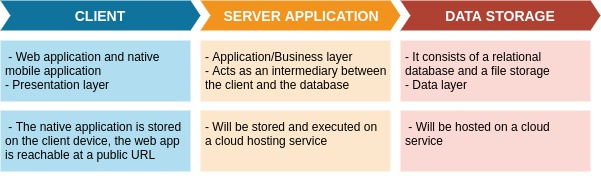
\includegraphics[origin=c,width=\textwidth]{DD_Images/Overview.jpg}
  \caption{\textit{Overview of the high-level components}}
\end{figure}